% --------------------------------------------------------------------
% LaTeX Template for Math Homework
% --------------------------------------------------------------------

\documentclass{article}

% --- PACKAGE IMPORTS ---
% These packages add functionality for math symbols, formatting, etc.
\usepackage[margin=.7in]{geometry}       % For setting page margins
\usepackage{amsmath, amssymb, amsthm}   % American Mathematical Society packages for advanced math
\usepackage{graphicx}                   % For including images
\usepackage{fancyhdr}                   % For creating custom headers and footers
\usepackage[colorlinks=true, urlcolor=blue, linkcolor=blue]{hyperref} % For clickable links
\usepackage{cancel}
\usepackage{array}
\usepackage{amsfonts}
\usepackage{amsxtra}
\usepackage{epsfig}
\usepackage{wasysym}
\usepackage{relsize}
\usepackage{tikz}
\tikzset{every picture/.style={scale=1.2}}
\renewcommand{\normalsize}{\fontsize{12}{20}\selectfont}



% custom commands
\newcommand{\myauthor}{Miguel Gomez}
\newcommand{\canceling}[2]{\textcolor{red}{\cancelto{\textcolor{black}{#1}}{\textcolor{black}{#2}}}}
\newcommand{\todo}[1]{\textcolor{blue}{TODO:#1}}

% --- DOCUMENT & AUTHOR INFORMATION ---
\title{Homework 1: Complex Numbers}
\author{
  MATH 3160\\
  \myauthor
}
\date{Completed: \today}

% --- HEADER & FOOTER CONFIGURATION ---
% This section sets up the header that will appear on each page.
\pagestyle{fancy}
\fancyhf{} % Clears the default header and footer
\lhead{Math 3160 -- HW 1} % Left side of header
\rhead{\myauthor} % Puts the author's name on the right side
\rfoot{Page \thepage} % Puts the page number on the bottom right

\begin{document}

\maketitle % This command generates the title based on the information above.

% ====================================================================
% --- START OF PROBLEMS ---
% ====================================================================

\section*{Problem 1: Complex Number Reduction}
Reduce each of these to a real number:
\begin{enumerate}
\item[(a)] $ \frac{1+2i}{3-4i} + \frac{2-i}{5i}$
  \begin{align*}
    \frac{1+2i}{3-4i} &+ \frac{2-i}{5i} = \\
    \frac{(1+2i)(3+4i)}{(3-4i)(3+4i)} &+ \frac{(2-i)(-5i)}{(5i)(-5i)} = \\
    \frac{(1+2i)(3+4i)}{9-16i^2} &+ \frac{(2-i)(-5i)}{-25i^2} = \\
    \frac{(3+4i+6i+8\canceling{-1}{i^2})}{9-16\canceling{-1}{i^2}} &+ \frac{(-10i+5\canceling{-1}{i^2})}{-25\canceling{-1}{i^2}} = \\
    \frac{(3+4i+6i-8)}{25} &+ \frac{(-10i-5)}{25} = \\
    \frac{(3+4i+6i-8)}{25} &+ \frac{(-10i-5)}{25} = \\
    \frac{(-5+10i)}{25} &+ \frac{(-10i-5)}{25} = \\
    \frac{(-5-5+10i -10i)}{25} = \boxed{-\frac{2}{5}}\\
  \end{align*}
\item[(b)] $ \frac{5i}{(1-i)(2-i)(3-i)}$
  \begin{align*}
    \frac{5i}{(1-i)(2-i)(3-i)} &=  \frac{5i}{(2-i-2i+i^2)(3-i)} = \\
    \frac{5i}{(2-i-2i+\canceling{-1}{i^2})(3-i)} &= \frac{5i}{(1-3i)(3-i)} = \\
    \frac{5i}{3-i-9i+3i^2} &= \frac{5i}{3-i-9i+3\canceling{-1}{i^2}}\ \ =\\
    \frac{5i}{3-i-9i-3} &= \frac{5i}{-10i} = \boxed{-\frac{1}{2}}\\
  \end{align*}
  \item[(c)] $ (1-i)^4$
    \begin{align*}
      (1-i)^4 &= \left(\frac{2}{\sqrt{2}}\right)^4\left(\frac{\sqrt{2}}{2}-\frac{\sqrt{2}}{2}i\right)^4 = \\
      \left(\frac{2}{\sqrt{2}}\right)^4\left(e^{-\frac{i\pi}{4}}\right)^4 &= \left(\frac{2}{\sqrt{2}}\right)^4 e^{-i\pi} = -\left(\sqrt{2}\right)^4 =-2^2= \boxed{-4}
    \end{align*}
\end{enumerate}

\vspace{.5cm} % Space for work

\hrule % Adds a horizontal line to separate problems.

\newpage
\section*{Problem 2: Vector Addition and Subtraction}
Locate the numbers $z_1+z_2$ and $z_1 - z_2$ vectorially by drawing a graph when:

\begin{enumerate}
    \item[(a)] $z_1 = 2i$, $z_2 = 2/3-i$
    
    \vspace{.5cm} % Space for graph
    
    \item[(b)] $z_1 = -\sqrt{3}+i$, $z_2 = \sqrt{3}$
    
    \vspace{.5cm} % Space for graph
    
    \item[(c)] $z_1 = (3,1)$, $z_2 = (1,4)$
    
    \vspace{.5cm} % Space for graph
    
    \item[(d)] $z_1 = x_1+iy_1$, $z_2 = x_1-iy_1$
    
    \vspace{.5cm} % Space for graph
\end{enumerate}
\hrule
\vspace{.5cm} % Space for graph
$z_1 = 2i$, $z_2 = 2/3-i$

\begin{center}
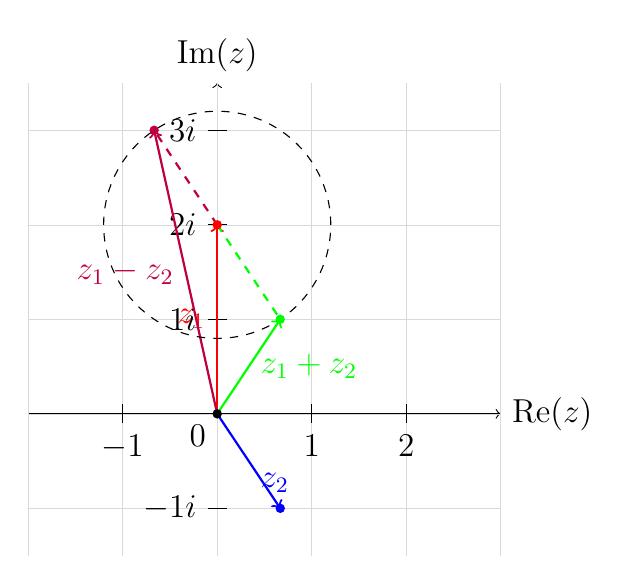
\begin{tikzpicture}
    % Draw axes
    \draw[->] (-2,0) -- (3,0) node[right] {$\text{Re}(z)$};
    \draw[->] (0,-1.5) -- (0,3.5) node[above] {$\text{Im}(z)$};
    
    % Grid
    \draw[gray!30, very thin] (-2,-1.5) grid (3,3.5);
    
    % Axis labels
    \foreach \x in {-1,1,2} {
        \draw (\x,0.1) -- (\x,-0.1) node[below] {$\x$};
    }
    \foreach \y in {-1,1,2,3} {
        \draw (0.1,\y) -- (-0.1,\y) node[left] {$\y i$};
    }
    
    % Define points
    \coordinate (z1) at (0,2);
    \coordinate (z2) at (0.667,-1);
    \coordinate (zsum) at (0.667,1);
    \coordinate (zsub) at (-0.667,3);
    
    % Draw vectors from origin
    \draw[->, thick, red] (0,0) -- (z1) node[midway, left] {$z_1$};
    \draw[->, thick, blue] (0,0) -- (z2) node[midway, below right] {$z_2$};
    \draw[->, thick, green] (0,0) -- (zsum) node[midway, right] {$z_1+z_2$};
    \draw[->, thick, purple] (0,0) -- (zsub) node[midway, left] {$z_1-z_2$};
    
    % Dashed lines from z1
    \draw[thick, dashed, green] (z1) -- (zsum);
    \draw[thick, dashed, purple] (z1) -- (zsub);
    
    % Circle centered at z1 with radius |z2|
    \draw[dashed, black] (z1) circle ({sqrt(0.667*0.667 + 1)});
    
    % Mark points
    \fill[red] (z1) circle (0.05);
    \fill[blue] (z2) circle (0.05);
    \fill[green] (zsum) circle (0.05);
    \fill[purple] (zsub) circle (0.05);
    
    % Origin
    \fill[black] (0,0) circle (0.05);
    \node[below left] at (0,0) {$0$};
\end{tikzpicture}

\end{center}
\newpage
$z_1 = -\sqrt{3}+i$, $z_2 = \sqrt{3}$

\begin{center}
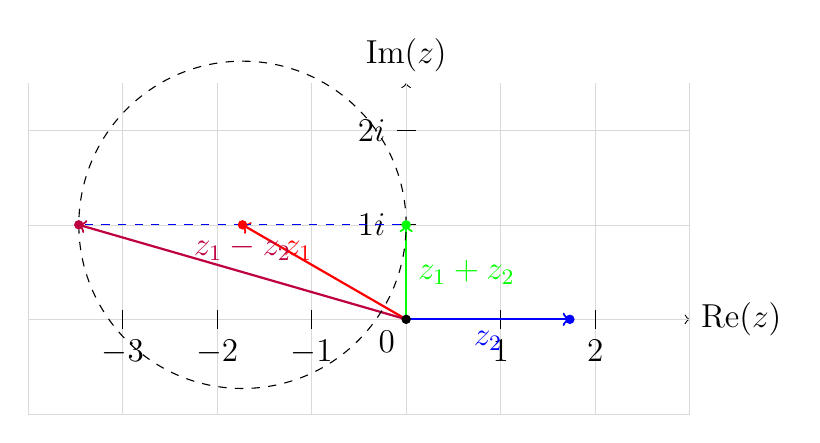
\begin{tikzpicture}
    % Draw axes
    \draw[->] (-4,0) -- (3,0) node[right] {$\text{Re}(z)$};
    \draw[->] (0,-1) -- (0,2.5) node[above] {$\text{Im}(z)$};
    
    % Grid
    \draw[gray!30, very thin] (-4,-1) grid (3,2.5);
    
    % Axis labels
    \foreach \x in {-3,-2,-1,1,2} {
        \draw (\x,0.1) -- (\x,-0.1) node[below] {$\x$};
    }
    \foreach \y in {1,2} {
        \draw (0.1,\y) -- (-0.1,\y) node[left] {$\y i$};
    }
    
    % Define points
    \coordinate (z1) at ({-sqrt(3)},1);
    \coordinate (z2) at ({sqrt(3)},0);
    \coordinate (zsum) at (0,1);
    \coordinate (zsub) at ({-2*sqrt(3)},1);
    
    % Draw vectors from origin
    \draw[->, thick, red] (0,0) -- (z1) node[midway, above left] {$z_1$};
    \draw[->, thick, blue] (0,0) -- (z2) node[midway, below] {$z_2$};
    \draw[->, thick, green] (0,0) -- (zsum) node[midway, right] {$z_1+z_2$};
    \draw[->, thick, purple] (0,0) -- (zsub) node[midway, above] {$z_1-z_2$};
    
    % Dashed lines from z1
    \draw[dashed, blue] (z1) -- (zsum);
    \draw[dashed, blue] (z1) -- (zsub);
    
    % Circle centered at z1 with radius |z2|
    \draw[dashed, black] (z1) circle ({sqrt(3)});
    
    % Mark points
    \fill[red] (z1) circle (0.05);
    \fill[blue] (z2) circle (0.05);
    \fill[green] (zsum) circle (0.05);
    \fill[purple] (zsub) circle (0.05);
    
    % Origin
    \fill[black] (0,0) circle (0.05);
    \node[below left] at (0,0) {$0$};
\end{tikzpicture}
\end{center}
\newpage
$z_1 = (3,1)$, $z_2 = (1,4)$

\begin{center}
  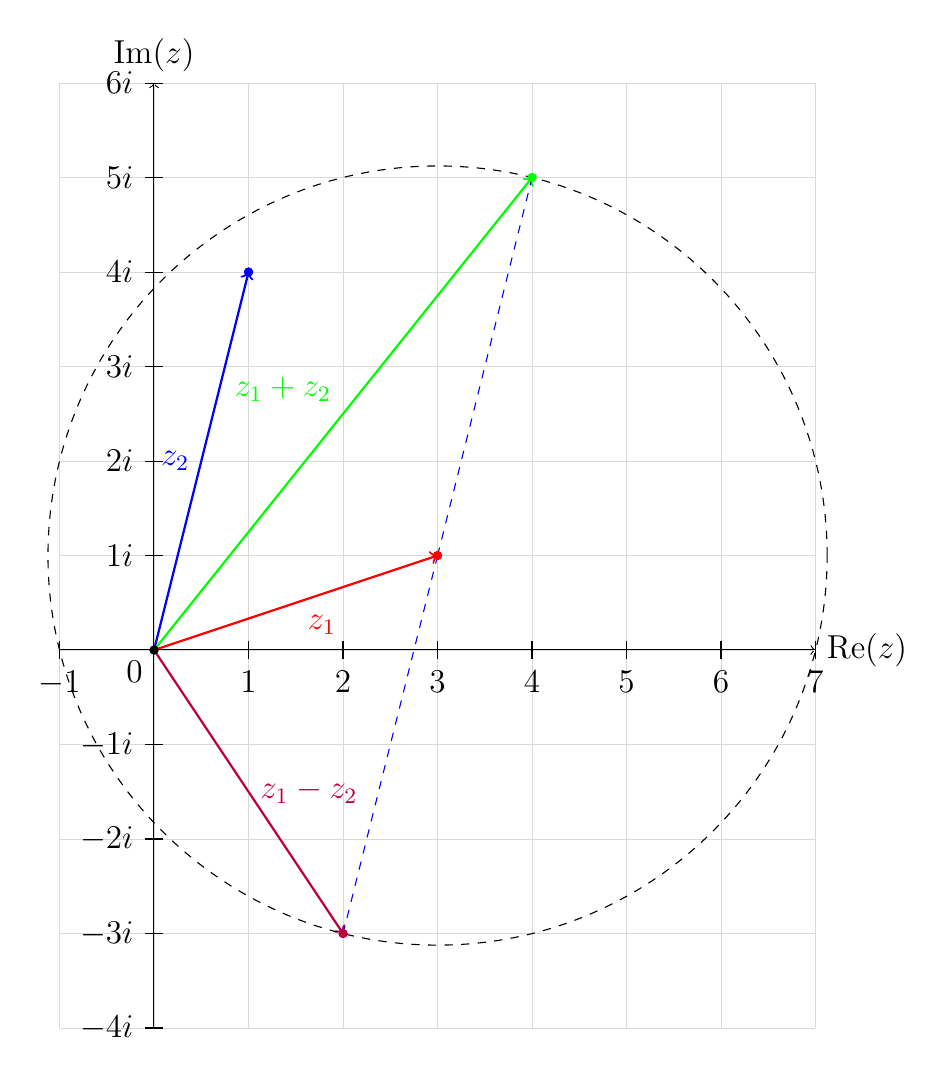
\begin{tikzpicture}
    % Draw axes
    \draw[->] (-1,0) -- (7,0) node[right] {$\text{Re}(z)$};
    \draw[->] (0,-4) -- (0,6) node[above] {$\text{Im}(z)$};
    
    % Grid
    \draw[gray!30, very thin] (-1,-4) grid (7,6);
    
    % Axis labels
    \foreach \x in {-1,1,2,3,4,5,6,7} {
        \draw (\x,0.1) -- (\x,-0.1) node[below] {$\x$};
    }
    \foreach \y in {-4,-3,-2,-1,1,2,3,4,5,6} {
        \draw (0.1,\y) -- (-0.1,\y) node[left] {$\y i$};
    }
    
    % Define points
    \coordinate (z1) at (3,1);
    \coordinate (z2) at (1,4);
    \coordinate (zsum) at (4,5);
    \coordinate (zsub) at (2,-3);
    
    % Draw vectors from origin
    \draw[->, thick, red] (0,0) -- (z1) node[midway, below right] {$z_1$};
    \draw[->, thick, blue] (0,0) -- (z2) node[midway, left] {$z_2$};
    \draw[->, thick, green] (0,0) -- (zsum) node[midway, above left] {$z_1+z_2$};
    \draw[->, thick, purple] (0,0) -- (zsub) node[midway, right] {$z_1-z_2$};
    
    % Dashed lines from z1
    \draw[dashed, blue] (z1) -- (zsum);
    \draw[dashed, blue] (z1) -- (zsub);
    
    % Circle centered at z1 with radius |z2|
    \draw[dashed, black] (z1) circle ({sqrt(17)});
    
    % Mark points
    \fill[red] (z1) circle (0.05);
    \fill[blue] (z2) circle (0.05);
    \fill[green] (zsum) circle (0.05);
    \fill[purple] (zsub) circle (0.05);
    
    % Origin
    \fill[black] (0,0) circle (0.05);
    \node[below left] at (0,0) {$0$};
\end{tikzpicture}
\end{center}
\newpage
$z_1 = x_1+iy_1$, $z_2 = x_1-iy_1$

\begin{center}
  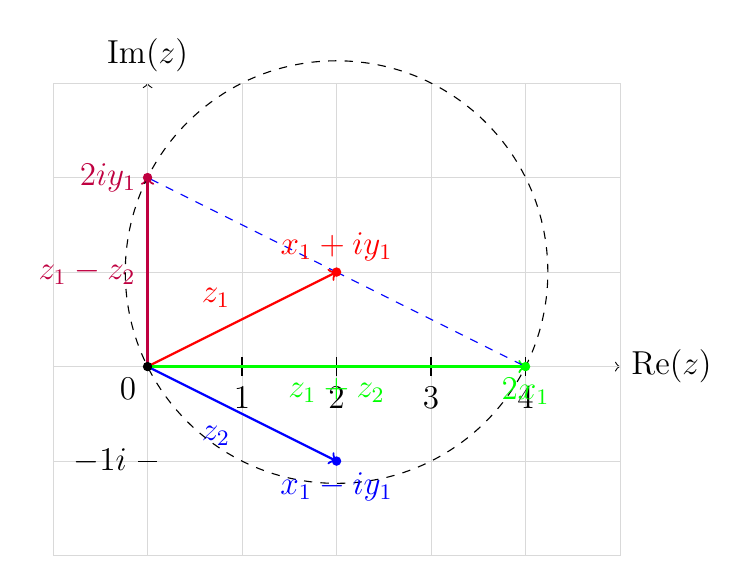
\begin{tikzpicture}
    % Draw axes
    \draw[->] (-1,0) -- (5,0) node[right] {$\text{Re}(z)$};
    \draw[->] (0,-2) -- (0,3) node[above] {$\text{Im}(z)$};
    
    % Grid
    \draw[gray!30, very thin] (-1,-2) grid (5,3);
    
    % Axis labels
    \foreach \x in {1,2,3,4} {
        \draw (\x,0.1) -- (\x,-0.1) node[below] {$\x$};
    }
    \foreach \y in {-1} {
        \draw (0.1,\y) -- (-0.1,\y) node[left] {$\y i$};
    }
    
    % Define points (using x1=2, y1=1)
    \coordinate (z1) at (2,1);
    \coordinate (z2) at (2,-1);
    \coordinate (zsum) at (4,0);
    \coordinate (zsub) at (0,2);
    
    % Draw vectors from origin
    \draw[->, thick, red] (0,0) -- (z1) node[midway, above left] {$z_1$};
    \draw[->, thick, blue] (0,0) -- (z2) node[midway, below left] {$z_2$};
    \draw[->, thick, green] (0,0) -- (zsum) node[midway, below] {$z_1+z_2$};
    \draw[->, thick, purple] (0,0) -- (zsub) node[midway, left] {$z_1-z_2$};
    
    % Dashed lines from z1
    \draw[dashed, blue] (z1) -- (zsum);
    \draw[dashed, blue] (z1) -- (zsub);
    
    % Circle centered at z1 with radius |z2|
    \draw[dashed, black] (z1) circle ({sqrt(5)});
    
    % Mark points
    \fill[red] (z1) circle (0.05);
    \fill[blue] (z2) circle (0.05);
    \fill[green] (zsum) circle (0.05);
    \fill[purple] (zsub) circle (0.05);
    
    % Origin
    \fill[black] (0,0) circle (0.05);
    \node[below left] at (0,0) {$0$};
    
    % Add labels for general case
    \node[red, above] at (z1) {$x_1+iy_1$};
    \node[blue, below] at (z2) {$x_1-iy_1$};
    \node[green, below] at (zsum) {$2x_1$};
    \node[purple, left] at (zsub) {$2iy_1$};
\end{tikzpicture}
\end{center}
\newpage
\section*{Problem 3: Geometric Sets in the Complex Plane}
In each case, sketch the set of points determined by the given condition:

\begin{enumerate}
    \item[(a)] $|z-1+i|=1$
    
    \vspace{.5cm} % Space for sketch
    
    \item[(b)] $|z+i| \leq 3$
    
    \vspace{.5cm} % Space for sketch
    
    \item[(c)] $|z-4i|\geq4$
    
    \vspace{.5cm} % Space for sketch
\end{enumerate}

\textit{Hint: Note that for any two complex numbers $z_1, z_2$, the absolute value $|z_1 - z_2|$ is the distance between $z_1$ and $z_2$ in the complex plane.}
\hrule
\vspace{.5cm} % Space for graph
$|z-1+i|=1$

\begin{center}
  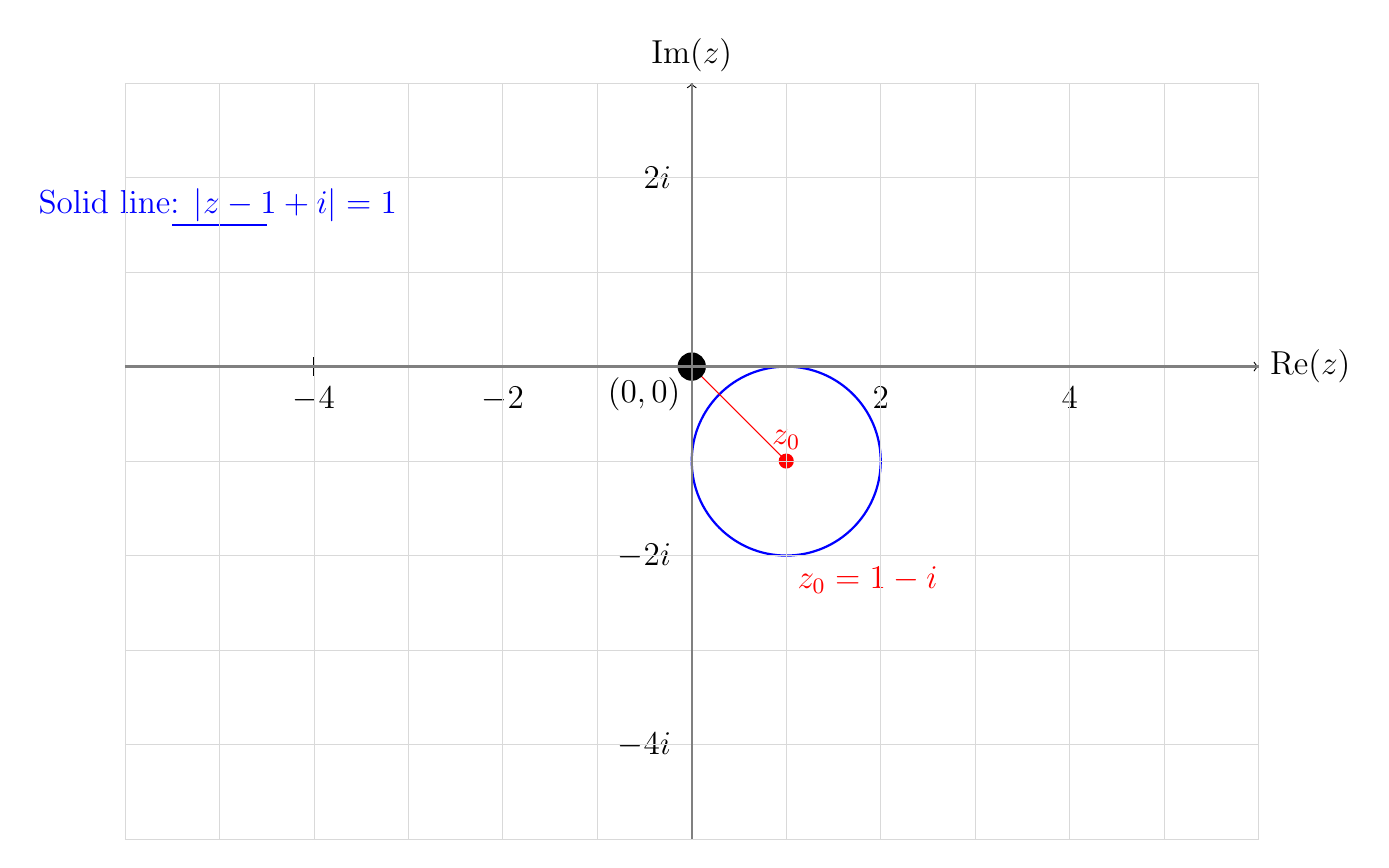
\begin{tikzpicture}
    
    % Draw axes
    \draw[->] (-6,0) -- (6,0) node[right] {$\text{Re}(z)$};
    \draw[->] (0,-5) -- (0,3) node[above] {$\text{Im}(z)$};
    
    % Add grid for better visualization
    \draw[gray!30, very thin] (-6,-5) grid (6,3);
    
    % Mark axis labels
    \foreach \x in {-4,-2,2,4} {
        \draw (\x,0.1) -- (\x,-0.1) node[below] {$\x$};
    }
    \foreach \y in {-4,-2,2} {
        \draw (0.1,\y) -- (-0.1,\y) node[left] {$\y i$};
    }
    
    % Define the center and radius
    \def\centerx{1}
    \def\centery{-1}
    \def\radius{1}
    
    % Shade the region inside the circle (|z+i| ≤ 3)
    %\fill[blue!20] (\centerx,\centery) circle (\radius);
    
    % Draw the circle boundary (solid line since it's ≤)
    \draw[thick, blue] (\centerx,\centery) circle (\radius);
    
    % Mark the center point
    \fill[red] (\centerx,\centery) circle (0.08);
    \node[red, below right] at (\centerx,\centery - 1) {$z_0 = 1-i$};
    \draw[red, ->] (0,0) -- (1,-1) node[above] {$z_0$};

    % Add radius line and label
    \draw[dashed, red] (\centerx,\centery) -- (\centerx,\centery+\radius);
    %\node[red, midway, right] at (0, 1) {$r = 3$};
    
    % Add title and condition
    %\node[above] at (-.5,2.25) {\textbf{Region: } $|z + i| \leq 3$};
    
    % Add legend
    \node[blue, below left] at (-3,2) {Solid line: $|z - 1 + i| = 1$};
    \draw[thick, blue] (-5.5,1.5) -- (-4.5,1.5);
    
    % Mark origin
    \fill[black] (0,0) circle (0.15);
    \node[below left] at (0,0) {$(0,0)$};
     % Add grid for better visualization
    \draw[gray!30, very thin] (-6,-5) grid (6,3);
    
    % Draw main axis lines
    \draw[gray, thick] (-6,0) -- (6,0);
    \draw[gray, thick] (0,-5) -- (0,3);
\end{tikzpicture}

\end{center}
\newpage
$|z+i| \leq 3$

\begin{center}
  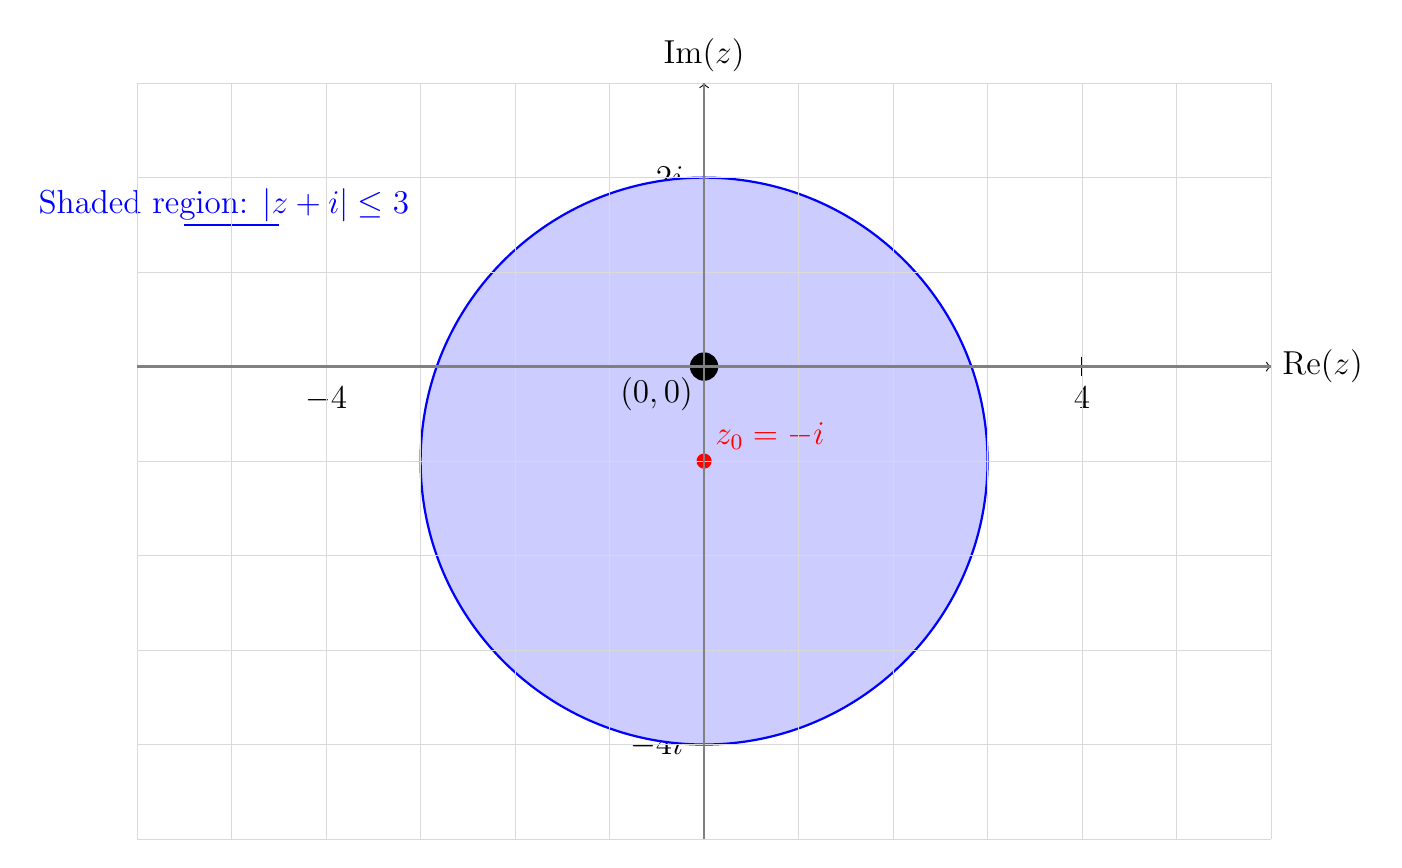
\begin{tikzpicture}
    
    % Draw axes
    \draw[->] (-6,0) -- (6,0) node[right] {$\text{Re}(z)$};
    \draw[->] (0,-5) -- (0,3) node[above] {$\text{Im}(z)$};
    
    % Add grid for better visualization
    \draw[gray!30, very thin] (-6,-5) grid (6,3);
    
    % Mark axis labels
    \foreach \x in {-4,-2,2,4} {
        \draw (\x,0.1) -- (\x,-0.1) node[below] {$\x$};
    }
    \foreach \y in {-4,-2,2} {
        \draw (0.1,\y) -- (-0.1,\y) node[left] {$\y i$};
    }
    
    % Define the center and radius
    \def\centerx{0}
    \def\centery{-1}
    \def\radius{3}
    
    % Shade the region inside the circle (|z+i| ≤ 3)
    \fill[blue!20] (\centerx,\centery) circle (\radius);
    
    % Draw the circle boundary (solid line since it's ≤)
    \draw[thick, blue] (\centerx,\centery) circle (\radius);
    
    % Mark the center point
    \fill[red] (\centerx,\centery) circle (0.08);
    \node[red, above right] at (\centerx,\centery) {$z_0 = -i$};
    
    % Add radius line and label
    \draw[dashed, red] (\centerx,\centery) -- (\centerx,\centery+\radius);
    %\node[red, midway, right] at (0, 1) {$r = 3$};
    
    % Add title and condition
    %\node[above] at (-.5,2.25) {\textbf{Region: } $|z + i| \leq 3$};
    
    % Add legend
    \node[blue, below left] at (-3,2) {Shaded region: $|z + i| \leq 3$};
    \draw[thick, blue] (-5.5,1.5) -- (-4.5,1.5);
    
    % Mark origin
    \fill[black] (0,0) circle (0.15);
    \node[below left] at (0,0) {$(0,0)$};
     % Add grid for better visualization
    \draw[gray!30, very thin] (-6,-5) grid (6,3);
    
    % Draw main axis lines
    \draw[gray, thick] (-6,0) -- (6,0);
    \draw[gray, thick] (0,-5) -- (0,3);
\end{tikzpicture}
\end{center}
\newpage
$|z-4i|\geq4$

\begin{center}
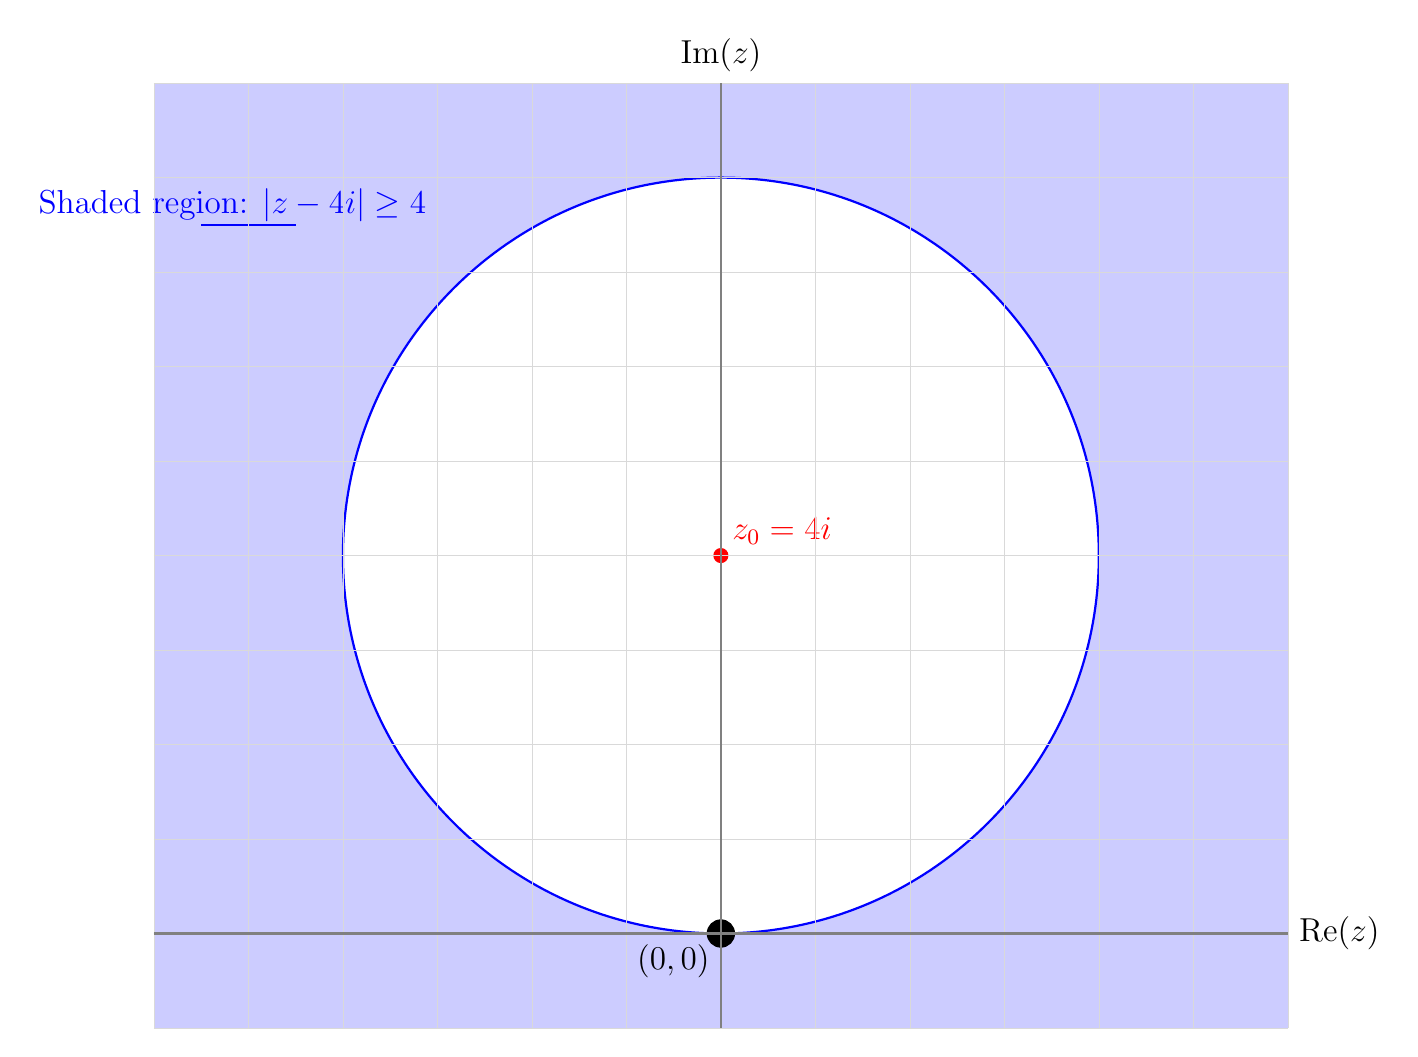
\begin{tikzpicture}
    
    % Draw axes
    \draw[->] (-6,0) -- (6,0) node[right] {$\text{Re}(z)$};
    \draw[->] (0,-1) -- (0,9) node[above] {$\text{Im}(z)$};
    
    % Add grid for better visualization
    \draw[gray!30, very thin] (-6,-1) grid (6,9);
    
    % Mark axis labels
    \foreach \x in {-4,-2,2,4} {
        \draw (\x,0.1) -- (\x,-0.1) node[below] {$\x$};
    }
    \foreach \y in {2,4,6,8} {
        \draw (0.1,\y) -- (-0.1,\y) node[left] {$\y i$};
    }
    
    % Define the center and radius
    \def\centerx{0}
    \def\centery{4}
    \def\radius{4}
    
    % Shade the region outside the circle (|z-4i| ≥ 4)
    % First, create a clipping path for the entire visible area
    \begin{scope}
        \clip (-6,-1) rectangle (6,9);
        % Shade everything
        \fill[blue!20] (-6,-1) rectangle (6,9);
        % Remove the interior of the circle (white fill)
        \fill[white] (\centerx,\centery) circle (\radius);
    \end{scope}
    
    % Draw the circle boundary (solid line since it's ≥)
    \draw[thick, blue] (\centerx,\centery) circle (\radius);
    
    % Mark the center point
    \fill[red] (\centerx,\centery) circle (0.08);
    \node[red, above right] at (\centerx,\centery) {$z_0 = 4i$};
    
    % Add radius line and label
    \draw[dashed, red] (\centerx,\centery) -- (\centerx,\centery-\radius);
    %\node[red, midway, right] at (0, 1) {$r = 4$};
    
    % Add title and condition
    %\node[above] at (-.5,7.75) {\textbf{Region: } $|z - 4i| \geq 4$};
    
    % Add legend
    \node[blue, below left] at (-3,8) {Shaded region: $|z - 4i| \geq 4$};
    \draw[thick, blue] (-5.5,7.5) -- (-4.5,7.5);
    
    % Mark origin
    \fill[black] (0,0) circle (0.15);
    \node[below left] at (0,0) {$(0,0)$};
     % Add grid for better visualization
    \draw[gray!30, very thin] (-6,-1) grid (6,9);
    
    % Draw main axis lines
    \draw[gray, thick] (-6,0) -- (6,0);
    \draw[gray, thick] (0,-1) -- (0,9);
\end{tikzpicture}

\end{center}  
\newpage
\section*{Problem 4: Principal Arguments}
preliminary necessary expressions:
  \begin{align*}
    \text{Arg}(z) &= \theta + 2\cdot pi\cdot k\ \ \ ;k\in \mathbb{Z} \\
    e^{i\theta} &= \cos\theta + i\sin{\theta}
  \end{align*}

Find the principal argument $\text{Arg}(z)$ when:

\begin{enumerate}
    \item[(a)] $z = \frac{i}{-2-2i}$
      \begin{align*}
        \frac{i}{-2-2i}\cdot\frac{-2+2i}{-2+2i} &= \frac{i(-2+2i)}{(-2-2i)(-2+2i)} = \\ 
        \frac{(-2i+2i^2)}{(4-4i+4i-4i^2)} &= \frac{(-2i+2\canceling{-1}{i^2})}{(4\canceling{0}{-4i+4i}-4\canceling{-1}{i^2})} = \\
        -\frac{2i+2}{8} &= -\frac{i+1}{4} = -\frac{i+1}{2\cdot 2} = \frac{1}{2}\cdot -\frac{1+i}{2}
      \end{align*}
      Introduce  a factor of $\sqrt{2}$ to top and bottom of fraction to convert into normalized vector
      \begin{align*}
        \frac{1}{2\sqrt{2}}\cdot -\frac{\sqrt{2}(1+i)}{2} & = \frac{1}{2\sqrt{2}}\cdot e^{-\frac{3\pi i}{4}}\\
        \therefore \text{Arg}(z) &= \boxed{-\frac{3\pi}{4}} 
      \end{align*}
    \item[(b)] $z = (\sqrt{3}-i)^6$
      
      For this one, we are already very close. We can just introduce a factor of 2 over 2 six times to be able to bring the half into the parentheses:    
\end{enumerate}

      \begin{align*}
        (\sqrt{3}-i)^6 &= \left(\frac{2}{2}\right)^6\cdot (\sqrt{3}-i)^6 =\\
        (2)^6\cdot \left(\frac{\sqrt{3}-i}{2}\right)^6 &= (2)^6\cdot  (e^{\frac{-i\pi }{\textcolor{red}{6}}})^{\textcolor{red}{6}} = 2^6\cdot e^{-i\pi}= 2^6\cdot e^{i\pi}\\
        \therefore \text{Arg}(z) &= \boxed{\pi}
      \end{align*}
\newpage
\section*{Problem 5: Argument Properties}

For any two non-zero complex numbers $z_1, z_2$, show that any angle $\theta$ in the set $\arg{(z_1z_2)}$ can be written as
\[ \theta = \theta_1 + \theta_2 \]
where $\theta_1 \in \arg(z_1)$ and $\theta_2 \in \arg(z_2)$. Also find an example where the principal argument $\text{Arg} (z_1z_2)$ is not equal to $\text{Arg} (z_1) + \text{Arg} (z_2)$.


Since we have two non-zero complex numbers, we can express them in exponential form:
$$z_1 = |z_1|e^{i\theta_1}, \quad z_2 = |z_2|e^{i\theta_2}$$
where $\theta_1 = \text{Arg}(z_1)$ and $\theta_2 = \text{Arg}(z_2)$.

Converting multiplication into addition in the exponent:
\begin{align*}
z_1z_2 &= |z_1||z_2|e^{i\theta_1} \cdot e^{i\theta_2} \\
&= |z_1||z_2|e^{i(\theta_1 + \theta_2)}
\end{align*}

Since for any complex number $z$, we have $\arg(z) = \text{Arg}(z) + 2\pi k$ where $k \in \mathbb{Z}$:
\begin{align*}
\theta_1 \in \arg(z_1) &\implies \theta_1 = \theta_1 + 2\pi k_1, \quad k_1 \in \mathbb{Z} \\
\theta_2 \in \arg(z_2) &\implies \theta_2 = \theta_2 + 2\pi k_2, \quad k_2 \in \mathbb{Z} \\
\theta \in \arg(z_1z_2) &\implies \theta = (\theta_1 + \theta_2) + 2\pi k, \quad k \in \mathbb{Z}
\end{align*}

Therefore, any angle $\theta \in \arg(z_1z_2)$ can be written as:
\begin{align*}
\theta &= (\theta_1 + 2\pi k_1) + (\theta_2 + 2\pi k_2) \\
 &= (\theta_1 + \theta_2) + 2\pi k\\
&= \theta_1 + \theta_2+ 2\pi k
\end{align*}
where we choose $k_1, k_2 \in \mathbb{Z}$ such that $k = k_1 + k_2$.

\newpage
\textbf{Example where } $\text{Arg}(z_1z_2) \neq \text{Arg}(z_1) + \text{Arg}(z_2)$\textbf{:}

\begin{align*}
z_1 &= e^{-i\pi/2}, \quad z_2 = e^{-i\pi/2} \\
\text{Arg}(z_1) &= -\frac{\pi}{2} \\
\text{Arg}(z_2) &= -\frac{\pi}{2} \\
\text{Arg}(z_1) + \text{Arg}(z_2) &= -\frac{\pi}{2} + \left(-\frac{\pi}{2}\right) = -\pi \\
\text{Since } -\pi &\notin (-\pi, \pi]: \\
\text{Arg}(z_1z_2) &= -\pi + 2\pi = \pi \\
\therefore \text{Arg}(z_1z_2) &\neq \text{Arg}(z_1) + \text{Arg}(z_2)
\end{align*}

\textbf{Note:} The principal arguments are equal, $\text{Arg}(z_1z_2) = \text{Arg}(z_1) + \text{Arg}(z_2)$, if and only if $\text{Arg}(z_1) + \text{Arg}(z_2) \in (-\pi, \pi]$. Otherwise, the sum must be adjusted by adding or subtracting $2\pi$ to bring it into the principal range.

\vspace{.5cm} % Space for proof and example

\hrule

\newpage
\section*{Problem 6: Principal Argument Addition}

Show that if $\text{Re}(z_1)>0$ and $\text{Re}(z_2)>0$, then $\text{Arg}(z_1z_2) = \text{Arg}(z_1)+\text{Arg}(z_2)$. Use polar form of $z_1$ and $z_2$ to do so.


Let $z_1 = |z_1|e^{i\theta_1}$ and $z_2 = |z_2|e^{i\theta_2}$ where $\theta_1 = \text{Arg}(z_1)$ and $\theta_2 = \text{Arg}(z_2)$.

Since $\text{Re}(z_1) = |z_1|\cos(\theta_1) > 0$ and $|z_1| > 0$, we have $\cos(\theta_1) > 0$.
Similarly, since $\text{Re}(z_2) = |z_2|\cos(\theta_2) > 0$ and $|z_2| > 0$, we have $\cos(\theta_2) > 0$.

For $\cos(\theta) > 0$ with $\theta \in (-\pi, \pi]$, we must have $\theta \in \left(-\frac{\pi}{2}, \frac{\pi}{2}\right)$.

Therefore:
\begin{align*}
\theta_1 &\in \left(-\frac{\pi}{2}, \frac{\pi}{2}\right) \\
\theta_2 &\in \left(-\frac{\pi}{2}, \frac{\pi}{2}\right) \\
\implies \theta_1 + \theta_2 &\in (-\pi, \pi)
\end{align*}

Since $\theta_1 + \theta_2 \in (-\pi, \pi) \subset (-\pi, \pi]$, no adjustment is needed, and:
$\text{Arg}(z_1z_2) = \theta_1 + \theta_2 = \text{Arg}(z_1) + \text{Arg}(z_2)$


\end{document}